%Results
\subsection{End-of-Round \BRAVO}
For the EoR \BRAVO simulations, our software estimated and used for each round
the round size that would achieve a $90\%$ probability of stopping if the true election outcome were as announced. In Figure \ref{fig:eor_bravo_sprob}, we display the proportion of EoR \BRAVO audits that stopped in the $j^{th}$ round
to all audits which had not yet stopped before the $j^{th}$ round, for only the first three rounds of the simulations because very few audits, $(.1)^{j-1}\cdot(10^4)$ on average, 
make it to the $j^{th}$ round. The proportions give an estimate
of the true probability of an EoR \BRAVO audit stopping in the $j$th round,
given that it has not already stopped in a previous round, when the underlying election is as announced. 
We see that, especially in earlier rounds for which 
the values are more representative of true audit behavior, 
our round size predictions are accurate.
In particular, the average across all margins is just above $.9=90\%$ for
all three rounds.

We also study the proportion of audits that stopped when the underlying election was a tie.
This proportion should approach a value less than the risk limit, $0.1$, as more audits are performed.

\begin{figure}
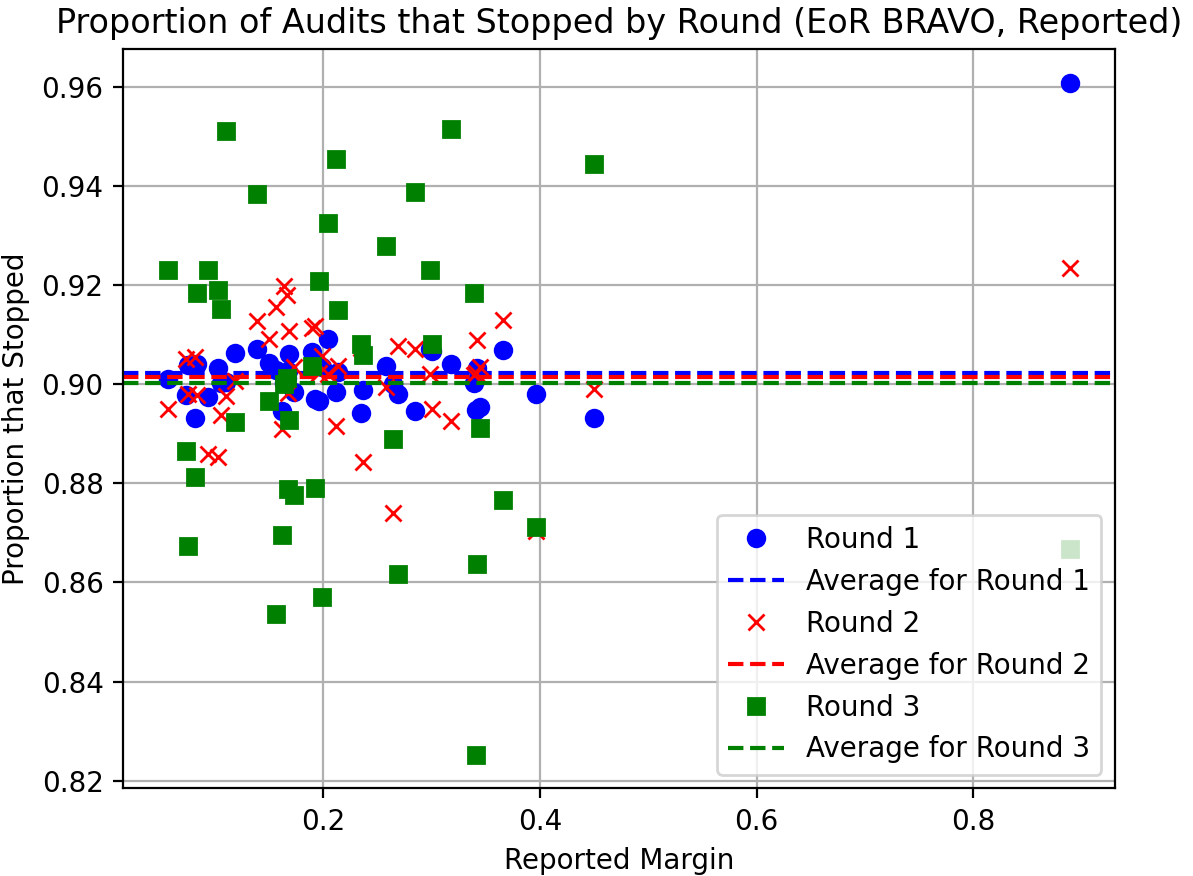
\includegraphics[width=0.8\textwidth]{eor_bravo_90perc_10^4_corrected/sprob_first_three_cropped.png}\caption{
This plot shows, for each state margin, when the underlying election is as announced, the number of EoR \BRAVO audits that stopped in the $j^{th}$ round,
as a fraction of all EoR \BRAVO audits which had not yet stopped before the $j^{th}$ round for $j=1,2,3$.}
\label{fig:eor_bravo_sprob}
\end{figure}

\begin{figure}
\includegraphics[width=0.8\textwidth]{eor_bravo_90perc_10^4_corrected/total_risk.png}
\caption{This plot shows, for each state margin,
the fraction of EoR \BRAVO audits that stopped in any of the $5$ rounds when the underlying election was a tie.}
\label{fig:eor_bravo_risk}
\end{figure}

We observe (see Figure~\ref{fig:eor_bravo_risk}) that the risk of EoR \BRAVO is roughly
an order of magnitude less than the risk limit. 
These results are as expected, because EoR \BRAVO is known to be too conservative \cite{usenix_minerva}.  

\subsection{Selection-Ordered \BRAVO}
% next_sample_size code is slow... tie simulations running still!
For the SO \BRAVO simulations, our software estimated and used for each round
the round size that would achieve a $90\%$ probability of stopping.

In Figure \ref{fig:so_bravo_sprob}, we again display proportions of SO \BRAVO audits that stopped in the $j^{th}$ round
to all audits which had not yet stopped before the $j^{th}$ round for only the first three rounds.
The proportions shown in Figure \ref{fig:so_bravo_sprob}, like those in \ref{fig:eor_bravo_sprob}, give an estimate
of the true probability of an SO \BRAVO audit stopping in the $j^{th}$ round,
given that it has not already stopped in a previous round. 
In \ref{fig:so_bravo_sprob}, we see that our round size predictions are relatively accurate,
all three rounds being near $90\%$.

\begin{figure}
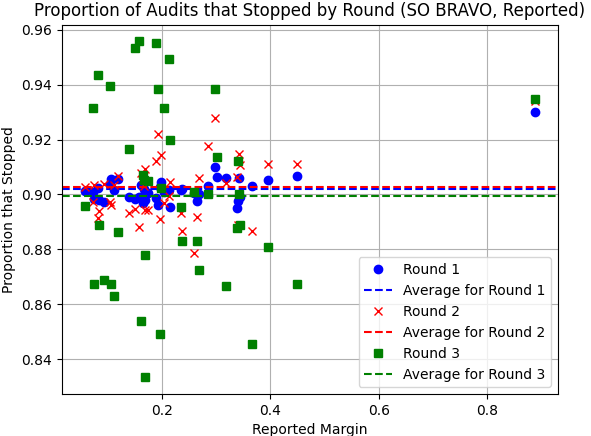
\includegraphics[width=0.8\textwidth]{so_bravo_90perc_10^4/sprob_first_three.png}\caption{
This plot shows, for each state margin, when the underlying election is as announced, the number of SO \BRAVO audits that stopped in the $j^{th}$ round,
as a fraction of all EoR \BRAVO audits which had not yet stopped before the $j^{th}$ round for $j=1,2,3$.}
\label{fig:so_bravo_sprob}
\end{figure}

As before, we will next consider the proportion of audits that stopped with an underlying tie over all five rounds.
This proportion, for a risk-limiting audit, should approach a value less than the risk limit, 
$0.1$, as more audits are performed.

In Figure~\ref{fig:so_bravo_risk} we show only the results for the $13$
states whose simulations with an underlying tie have finished running.
To estimate the next round size that achieves a desired stopping probability,
the SO \BRAVO software generates the probability distribution on the number of ballots in the sample ballot by ballot (see \cite{usenix_minerva}) since
the stopping condition needs to be evaluated for each individual ballot drawn.
because the underlying tied election causes audits to move on to larger rounds, 
the simulations are computationally expensive. SO \BRAVO is proven to be a Risk-Limiting Audit,
and we observe in Figure~\ref{fig:so_bravo_risk},
that the risk of SO \BRAVO is much
nearer the risk limit than that of EoR \BRAVO, as expected. 

\begin{figure}
\includegraphics[width=0.8\textwidth]{so_bravo_90perc_10^4/total_risk.png}
\caption{This plot shows, for each state margin,
the fraction of SO \BRAVO audits that stopped in any of the $5$ rounds when the underlying election was a tie.}
\label{fig:so_bravo_risk}
\end{figure}

%TODO SO and EoR macros

\subsection{\Minerva Simulations}
The proof that \Minerva is an RLA \cite{usenix_minerva} assumes that the round schedule is pre-determined. For this reason, we have to choose the round sizes of a \Minerva 
audit {\em a priori}.
For this paper, we consider two choices of round sizes.
For both, we estimate and use a first round size 
for
a $90\%$ probability of stopping.
Then, for subsequent rounds, we either (i) 
draw the same number of ballots in each round or (ii)
multiply the previous round size by a factor of $1.5$ and 
sample this many new ballots.
We consider the case of drawing samples of the same size
because it may reflect a practical way to continue an
audit; if election officials have selected some first round size within
reasonable logistical bounds, drawing the same number of 
ballots in subsequent rounds may be practical.
We also consider round sizes with samples increasing by a multiple
of $1.5$ because this multiple gives a very rough approximation of 
round sizes with a $90\%$ probability of stopping for \Minerva. 

As with the preceding simulations, we ran $10,000=10^4$ trials
per state for both an underlying election as reported and an underlying tied election. 

Figure~\ref{fig:minerva1_sprob} and Figure~\ref{fig:minerva1p5_sprob} show that the first round size estimates were fairly accurate for multipliers of $10.$ and $1.5$ respectively, with first round stopping probabilities being very close to $90\%$. For subsequent rounds, the multipliers of $1.0$ and $1.5$ respectively did not consistently achieve $90\%$ stopping
probability, as they were not accurate estimates of $90\%$ stopping probabilities. Note that we chose a simple multiplier for future rounds, but one could make more accurate round size estimates before the audit begins. 

\begin{figure}
\includegraphics[width=0.8\textwidth]{minerva_multiround_1x_10^4/sprobs_first_three.png}
\caption{This plot shows, for each state margin, when the underlying election is as announced, the number of \Minerva audits that stopped in the $j^{th}$ round,
as a fraction of all \Minerva audits which had not yet stopped before the $j^{th}$ round for $j=1,2,3$ and round size multiple of $1.0$.}
\label{fig:minerva1_sprob}
\end{figure}

\begin{figure}
\includegraphics[width=0.8\textwidth]{minerva_multiround_1p5x_10^4/sprobs_first_three.png}
\caption{This plot shows, for each state margin, when the underlying election is as announced, the number of \Minerva audits that stopped in the $j^{th}$ round,
as a fraction of all \Minerva audits which had not yet stopped before the $j^{th}$ round for $j=1,2,3$ and round size multiple of $1.5$.}
\label{fig:minerva1p5_sprob}
\end{figure}

Figures \ref{fig:minerva1_risk} and Figure~\ref{fig:minerva1p5_risk} show that fewer than $0.1$ of the audits stopped when the underlying election was a tie, for round multiples of $1.0$ and $1.5$ respectively, as would be expected for an RLA with risk limit $0.1$. 
Unlike EOR \BRAVO, the experimental risks here are much closer to the risk limit,
showing that \Minerva stops on average with a less conservative risk; \Minerva is sharper.

\begin{figure}
\includegraphics[width=0.8\textwidth]{minerva_multiround_1x_10^4/total_risk.png}
\caption{This plot shows, for each state margin,
the fraction of \Minerva audits with a round size multiple of $1.0$ that stopped in any of the $5$ rounds when the underlying election was a tie.}
\label{fig:minerva1_risk}
\end{figure}

%For the Minerva simulations with a round size multiple of $1.5$,
%we increased the number of simulations to $10^6$ per state for 
%both an underlying tie and underlying announced outcome. 

%\includegraphics[width=\textwidth]{minerva_multiround_1p5x_10^6/total_risk.png}

% we could suggest that predicting accurate multiples is possible (same curve rather than line)

\begin{figure}
\includegraphics[width=0.8\textwidth]{minerva_multiround_1p5x_10^4/total_risk.png}
\caption{This plot shows, for each state margin,
the fraction of \Minerva audits with a round size multiple of $1.5$ that stopped in any of the $5$ rounds when the underlying election was a tie.}
\label{fig:minerva1p5_risk}
\end{figure}




